\documentclass{article}
\usepackage[utf8]{inputenc}

\usepackage{enumitem} % itemize com a b c 

\title{Desafio Arquiteto Cloud}
\author{Rodolfo Labiapari Mansur Guimarães \\\href{mailto:rodolfolabiapari@gmail.com}{\texttt{rodolfolabiapari@gmail.com}}}
\date{Belo Horizonte - MG, \today}

\usepackage{natbib}
\usepackage{graphicx}
\usepackage{hyperref}

\begin{document}

\maketitle

\section{Introdução}

Data da entrega: 28/09 Segunda-feira

Dúvidas ou perguntas enviar para \href{mailto:desafio-vagas@solvimm.com}{desafio-vagas@solvimm.com} e copiar \\\href{mailto:roberta@huntingti.com}{roberta@huntingti.com}.

Favor confirmar o recebimento deste e-mail.

O cenário hipotético para o desafio do processo seletivo para Analista de Infra Cloud será o descrito abaixo:

\subsection{Desafio}
O cliente Escola na Nuvem precisa migrar a sua plataforma Moodle de ensino à distância para a AWS. Segundo o diretor de TI da empresa, o Severino Santos, hoje estão na LocaWeb, com aplicação e banco de dados em um único servidor com 8 CPU e 16 GB de RAM, mas normalmente utiliza na faixa de 30\% dos recursos, tendo picos imprevisíveis que chegam a 100\%, às vezes até ficando fora do ar, o que fez a empresa perder cerca de 20\% de alunos nesse último ano. A aplicação possui 200 GB de disco, sendo que 150 GB são de imagens e vídeos. O próximo semestre letivo começa em fevereiro de 2019 e eles precisam ter o ambiente em produção até 1 mês antes.

A empresa estruturou muitos novos cursos, que serão anunciados ao longo do primeiro semestre de 2019, tendo uma previsão de aumento de alunos da ordem de 50\% no final do ano, em relação ao início do semestre. O diretor está preocupado com esse crescimento frente aos desafios que tiveram na LocaWeb esse ano. Portanto, ele entrou em contato com a Amazon Web Services, o maior provedor de computação em nuvem do mundo, para entender como a Escola na Nuvem pode se beneficiar da nuvem. A AWS nos encaminhou o cliente para que possamos projetar a jornada de adoção para a nuvem da empresa e oferecermos uma solução para o Severino Santos.

Sendo assim, será importante planejar o processo de migração, e também planejar e dimensionar a infraestrutura, podendo consultar a documentação da AWS. Para os elementos de infraestrutura, é importante utilizar a nomenclatura da AWS, tanto para os serviços (Ex.: EC2) quanto para as configurações (Ex.: EC2 de 1 CPU e 1 GB de RAM é a t2.micro).

É importante realizar uma estimativa de custos na AWS, utilizando a AWS Calculator.

Lembramos que será importante pensar nos princípios de segurança, disponibilidade, escalabilidade e custo e explicar como eles compõem a arquitetura. Além disso, é preciso explicar como que o Moodle propriamente dito fará uso desses serviços, pois não basta só criar os elementos na arquitetura da AWS, são necessárias algumas configurações no Moodle para utilizar alguns serviços específicos que são importantes nessa arquitetura.

Por fim, será preciso projetar uma solução de monitoramento dessa infraestrutura, bem como definir como será feito o processo de atualização (deploy de novas versões) do Moodle após implantação, pois após a utilização em produção, o cliente espera que o sistema não saia do ar, mesmo quando estiver ocorrendo uma atualização.

\subsection{Entrega}
Para o desafio, teremos 2 entregáveis:
\begin{itemize}
    \item Um e-mail para o arquiteto que fará a validação da arquitetura proposta, com uma representação da arquitetura (sugerimos usar alguma ferramenta como o Draw.io ou Cloudcraft, mas podem buscar outras opções), um texto explicando o que representa cada elemento presente e sua funcionalidade para o sistema, bem como possíveis especificidades de integração com o Moodle. Nesse e-mail, serão apresentadas também a solução de monitoramento e a estratégia de atualização da plataforma
    \item Um e-mail para o cliente, falando do processo de migração (as etapas envolvidas) a estimativa de custos da infraestrutura na AWS e um cronograma macro. Nesse ponto, não é necessário falar de muitos detalhes técnicos com o cliente, mas é importante deixar claro para o cliente as vantagens da arquitetura proposta e tranquilizá-lo quanto aos problemas que ele possui no provedor atual. Por fim, é muito importante a cordialidade e o bom atendimento ao cliente.
\end{itemize}

Esses dois e-mails devem vir em arquivos anexos enviados para um único e-mail em resposta a este desafio.





\section{E-mail para o Arquiteto}
Caro arquiteto.

Depois de estudado a atual arquitetura do cliente e a aplicação que ele utiliza, percebo que baseia-se na simples situação do usuário que necessitar conectar a um servidor na internet fazendo uma simples autenticação e consumo de conteúdo dentro da plataforma, envolvendo um servidor e um banco de dados no caso mais básico. Entretanto, utilizando os vários serviços disponíveis pela AWS, podemos trazer inúmeras melhorias para esse cliente e vou discuti-las no decorrer deste relatório.

Proponho duas soluções para que sejam discutidas tanto com nossa equipe técnica e com o cliente para obtermos o resultado que mais atenderá suas necessidades hoje e suas futuras perspectivas para seu sistema.

A primeira aqui apresentada é uma solução que aproxima bastante da atual realidade do cliente, já a segunda, proponho a troca da arquitetura para uma que utiliza-se de containers. 
As duas compartilham, de modo geral, os mesmos serviços e recursos vista de uma forma ampla, com exceção do servidor distribuído onde o Moodle será depositado. 
Para maior compreensão, será explicado primeiramente o que as duas possuem de comum e depois passarei por cada uma, separadamente, explicando seus diferenciais.

\subsection{Visão Geral dos Recursos e Serviços Utilizados em Ambas as Soluções}

% geralzao
Para as arquiteturas que aqui proponho, precisamos de alguns recursos que serão utilizado em ambas as soluções e esses recursos são descritos a seguir.

Nelas temos incluso um LoadBalancer para distribuição das requisições para o servidor que será distribuído em zonas distintas, um banco de dados para dados relacionais e também um banco de caches, ambos gerenciados pela AWS. 
Um sistema de arquivos compartilhado para arquivos acessados pelos servidores e por fim, um CDN à arquitetura. 

Também incluo alguns itens mais específico como um serviço de monitoramento e de auditoria além da contratação de um suporte nível básico da nuvem para facilitar a abertura de chamados quando necessário. Um serviço de DNS e certificados gerenciados também farão parte dos serviços que serão contratados.

Dessa forma seria utilizado os seguintes serviços da AWS:

\begin{itemize}
    \item \textbf{AWS Route53 e AWS Certificate Manager:} \textit{Configuração dos domínios utilizados para o sistema e certificados;}
    
    \item \textbf{AWS CloudFront:} \textit{CDN gerenciado pela AWS para distribuição de conteúdo frequentemente requisitado do Moodle. Um dos maiores ganhos é a redução de latência do cliente ao acessar o sistema;}

    \item \textbf{AWS Application Load Balancer:} \textit{Roteamento na camada 7 de requisições para o sistema que estará dividido por zonas independentes;}
    
    \item \textbf{AWS RDS:} \textit{Banco de dados gerenciado pela AWS, replicado, para armazenamento de dados relacionais; A configuração inicial proposta para o cliente é um Amazon Aurora PostGres com instância do tipo \textit{db.r5.large} de 100GB com a replicação habilitada e \textit{snapshots} diários para backup. Dependendo da análise de uso do banco, podemos aumentar o tamanho do disco proporcionando maior performance do banco em IOPs.}

    \item \textbf{AWS ElastiCache:} \textit{Como tratamos de uma aplicação que utiliza sessões e caches, um serviço que poderia fazer armazenamento desses dados seria o ElastiCache aumentando a performance sistêmica; Utilizaríamos um serviço com instância do tipo \textit{t3.medium}, replicado, seria necessário uma análise mais profunda para a determinação da instância ideal.}

    \item \textbf{AWS EFS:} \textit{Serviço de sistema de arquivos para uso compartilhado dos dados; O armazenamento proposto é de 150GB inicialmente.}
    
    \item \textbf{AWS S3:} \textit{Armazenamento dos estados do Terraform.}
    
    \item \textbf{AWS CloudTrail:} \textit{Para auditorias.}
    
    \item \textbf{Suporte AWS:} \textit{Suporte AWS, nível Developer, para facilidade em abertura de chamados na AWS.}
\end{itemize}

Descrito os recursos comuns entre as soluções, iniciarei a descrição do primeiro modelo de servidor, utilizando instâncias EC2.

\subsection{Solução utilizando AWS EC2 AutoScaling}

Para a solução que utiliza-se de AWS EC2 Autoscaling indico duas formas de provisionar as instâncias de forma automática e escalável:

\begin{enumerate}
    \item \textbf{UserData:} Poderiamos utilizar o recursos de instalação no boot quando as instâncias iniciarem fazendo um \textit{script} que sempre baixa o Moodle via git e configura os diretórios. Entretanto não considero essa forma a melhor prática mais deixo aqui como sugestão para discussão;
    \item \textbf{Packer:} Outra forma seria construir imagens com todos os recursos que precisamos nela já instalados e prontos para uso utilizando o AWS AMI Builder (Packer). As vantagens em utilizar esse processo são:
    \begin{itemize}
        \item Versionamento das imagens utilizadas e facilidade em atualização de sistema alterando somente o AWS AutoScale para a nova imagem;
        \item Provisionamento mais rápido já que os recursos já estão todos instalados e pronto para uso;
        \item Facilidade de \textit{rollback} para uma imagem antiga;
        \item Segurança já que as AMIs são privadas e estão fechadas para alterações.
    \end{itemize}
\end{enumerate}

O esquema utilizando AWS EC2 AutoScaling proposto está disponível na Figura~\ref{fig:ec2} abrangendo todos os serviços descritos.
\newpage
\begin{figure}[h!]
\centering
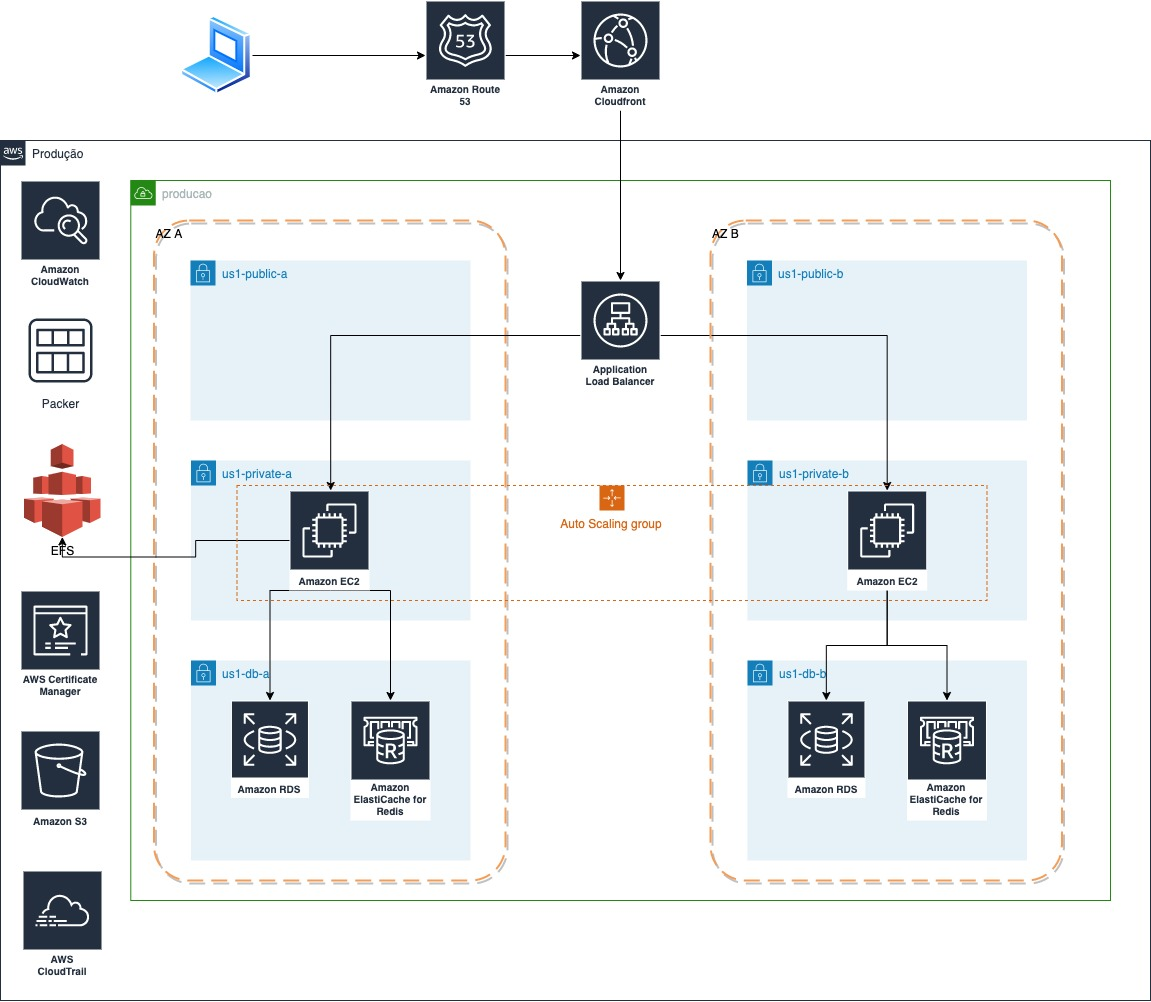
\includegraphics[scale=0.3]{ec2}
\caption{Diagrama do projeto utilizando EC2 Escalado.}
\label{fig:ec2}
\end{figure}

E a configuração proposta para essas instâncias EC2 seria:

\begin{itemize}
    \item \textbf{AWS EC2 com AutoScaling:} \textit{Instâncias EC2 com AutoScale habilitado utilizando ou UserData ou Packer; Proponho o uso de EC2 m5.large com 50GB\footnote{Fonte: \url{https://docs.moodle.org/39/en/Installing_Moodle}}.}
\end{itemize}

\subsection{Solução utilizando AWS ECS}

A segunda arquitetura que proponho seria baseada em containers visto que a Bitname disponibiliza\footnote{Disponível em: https://hub.docker.com/r/bitnami/moodle} o Moodle em Docker Container.

Dessa forma, ao invés de utilizar instâncias EC2 escaladas, utilizaríamos um serviço de container gerenciado como o ECS junto com o ECR para armazenamento das imagens dos containers versionados.
Configuraríamos o container para apontar seus volumes para os respectivos serviços mencionados.

O esquema proposto para esta arquitetura está disponível na Figura~\ref{fig:container} e os recursos da AWS que serão utilizados nessa estratégia estão descritos em seguida.

\begin{figure}[h!]
\centering
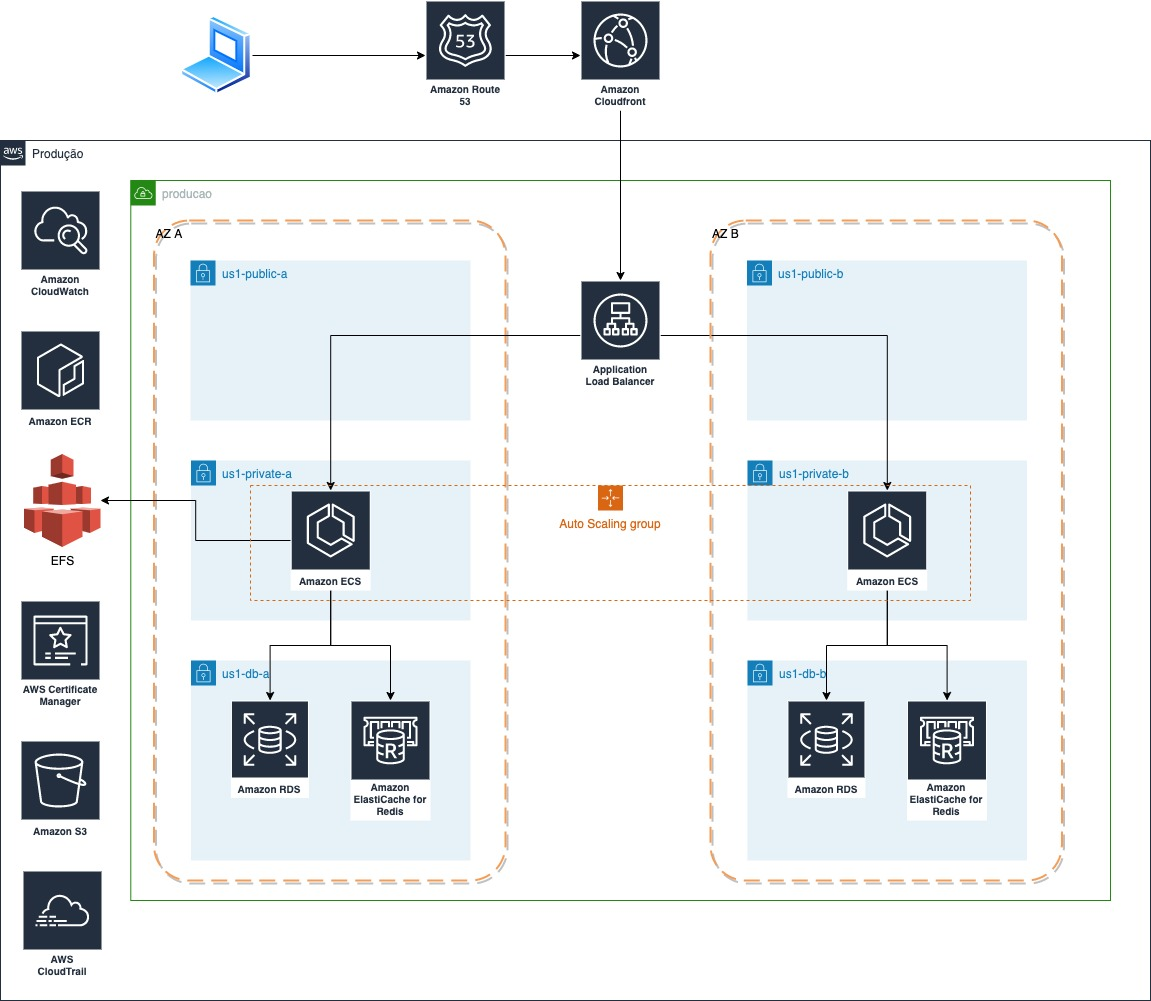
\includegraphics[scale=0.30]{ecs}
\caption{Diagrama do projeto utilizando ECS Escalado.}
\label{fig:container}
\end{figure}

\begin{itemize}
    \item \textbf{AWS ECR:} \textit{Serviço para o armazenamento dos containers versionados por tags, criando uma fonte sólida, sempre disponível para uso privado do sistema Moodle;}

    \item \textbf{AWS ECS:} \textit{A Amazon disponibiliza uma gama de serviços para podermos utilizar containers. O ECS é um serviço que enquadra nesse caso pois é de fácil para uso e manutenção e atualização, além de disponibilizar recursos de monitoramentos e escalabilidade integrados ao serviço; Como não tenho dados de uso do sistema atual proponho o uso de EC2 \textit{m5.large}, escalado automaticamente com 50GB.}
\end{itemize}


\subsection{Monitoramento}
O monitoramento destes recursos é facilmente obtido utilizando o serviço AWS CloudWatch.

% geralzao de monitoramento
O AWS CloudWatch possui integração com os recursos da AWS podendo criar um painel de monitoramento com todas as informações dos recursos utilizados como AWS RDS, AWS CloudFront e o AWS ECS ou EC2s.

% cloud logs e alertas
Além de monitoramento de recursos AWS, teremos também o CloudWatch Logs na qual receberá logs das Tasks do ECS ou dos EC2 utilizando um agente instalado manualmente podendo ser enviado para um S3 para uma retenção maior.
Além de logs pode-ser configurar alertas para notificação em casos fora do atípico.

\subsection{Atualização da Plataforma para Cloud}
Aqui será descrito como a atualização da plataforma será realizada, saindo da plataforma atual e migrando tudo para a nuvem.
O processo de migração baseará na documentação oficial do Moodle e também utilizarei o diretório base \texttt{/\$\{path\}/moodle} como exemplo.

\subsubsection{Janela de Manutenção e Backups}
% janela
O primeiro passo é determinar com o cliente uma janela para que esse processo seja feito. 

%modo manutencao
Nesta janela, deve-se primeiro ativar o Moodle em modo de manutenção, impedindo novos usuários acessarem a plataforma.

%backup
Feito isso, a primeira tarefa seria realizada sobre o banco de dados.
Dessa forma, iniciaria-se um backup do banco fazendo um \textit{dump} dele.
Além do banco de dados, seria feito o backup dos diretórios onde o código do sistema, arquivos e os caches estão salvos.

\subsubsection{Migração do banco de dados}

%migracao do banco de dados usando dump
%Com o banco de dados salvo, inicia-se o processo de migração para a nuvem. Utilizando o mesmo \textit{dump}, popularíamos o banco foi instanciado na nuvem.

% rds
Utilizando o serviço da AWS chamado AWS DMS, que automatiza o processo de migração de bases para a nuvem, inicia-se-á a cópia dos dados relacionais para o AWS RDS.

% configuracao do memcached
Para a configuração dos diretórios \texttt{/\$\{path\}/moodle/\{cache,temp\}} onde ficarão os arquivos de cache, configura-se o AWS ElastiCache para o seu armazenamento.

% efs
Os arquivos que serão compartilhados entre todos os servidores distribuídos, utilizará o AWS EFS para armazenamento distribuído.
Esse diretório é representado pelo \texttt{/\$\{path\}/moodle/data}. 
Montaria-se apontando para o AWS EFS e carregaríamos os arquivos antigos para esse novo diretório.

% migração do moodle
Em seguida configuraríamos o código do sistema (caso a arquitetura final for a de AWS EC2 AutoScaling).
O local ideal para armazenar esses arquivos é o no próprio \textit{root} da instância e por isso a instalação seria realizado nestes diretórios que estão localizados na instância \texttt{/\$\{path\}/moodle/\{local,html\}}.
Para imagens de containers essa configuração já estará definida previamente no momento de \textit{build}.


% sudo install
%Configurado todos esses recursos, executaríamos a instalação do sistema e testaríamos o seu sucesso.

% reaponta o dns
Depois de testado e aprovado o funcionamento do sistema, pode-se então alterar o DNS apontado ainda para o servidor antigo, para o Load Balancer que distribuirá o tráfego para os novos servidores distribuídos na nuvem.

Por fim, retira-se o modo manutenção do Moodle e monitora-se por um período de tempo (alguns dias) a fim de certificar o funcionamento deste.

Após todo este processo desliga-se por completo o sistema antigo do cliente.


\section{E-mail para o cliente}
À Escola na Nuvem.

% falando dos problemas
Fizemos uma análise em seu ambiente atual e por mais que ele esteja funcional na maioria do tempo, ele não é confiável, escalável ou robusto.
Entretanto, essas qualidades podem ser obtidas com bastante facilidade ao utilizar os recursos e serviços hoje oferecidos pela computação em nuvem.

% falando do que será feito
Dessa forma, propomos inicialmente a separação de dados e códigos, colocando seu banco de dados, sistema de arquivos, caches e o sistema Moodle em serviços separados permitindo maior autonomia e facilidade de gerência de cada um deles. 
Também implantaremos uma arquitetura de servidores escaláveis, também gerenciados, para suportar todas as requisições em momentos de pico e bem como reduzir os custos quando o Moodle não é utilizado por seus usuário como os horários de madrugada, por exemplo. 
Esse disposição sistêmica permite ainda a fácil manutenção e futuras atualizações.

% pulo pro próximo capitulo

Primeiro será provisionado todo seu ambiente em nuvem construindo as instâncias de banco de dados, de banco de caches, sistema de arquivos e de seu servidor distribuído para que logo possamos iniciar a migração para essas instâncias.
O processo de migração, junto à estimativa de custo e o cronograma planejado para provisionamento, migração e desligamento do servidor antigo são descritos a seguir.


\subsection{Processo de Migração}

A migração será realizado por etapas.

Utilizaremos uma janela de manutenção definida junto com vocês para que esses processos de backup e migração sejam realizados com segurança.

Primeiro faremos a migração do banco de dados e em seguida a instalação e configuração final do Moodle nos servidores copiando as imagens e vídeos para o novo sistema de arquivos, todos esses recursos distribuídos na nuvem.

Por precaução, pedimos que, mesmo com o sucesso da migração, deixemos seu ambiente antigo ainda em funcionamento por cerca de uma semana para garantir um \textit{rollback} rápido e seguro caso algum imprevisto aconteça. 
Passado este período de provação, executando o novo servidor na nuvem, podemos desligar o servidor antigo com segurança.

\subsection{Custo estimado}

Também fizemos uma estimativa de custo sobre a arquitetura proposta. 
Lembramos que esses tipos de instâncias que foram provisionadas na nuvem podem ser alteradas futuramente para adequar a sua real necessidade a partir da métricas que vamos obter com as análises de uso de requisições no Moodle que a nuvem nos proporcionará além de banco de dados e outros. 
Outro detalhe é que exibiremos um valor \textit{on-demand} e outro utilizando \textit{upfront} que é um contrato prolongado, podendo assim dizer, com a nuvem que pode reduzir o seu gasto visto que ele funciona como um adiantamento por um determinado tempo de uso pelos recursos contratados. 

Esclarecidos esses pontos, os planos são apresentados a seguir.

\subsubsection{\textit{On-Demand}}

Sem o uso de um \textit{upfront} (ou seja, sem um contrato com a nuvem), estimamos um valor aproximado de \texttt{816.91 USD} mensal, dando um total anual de \texttt{9,802.97 USD}\footnote{Calculadora disponível no endereço: \url{https://calculator.aws/\#/estimate?id=06adb73e7aab34bf9dc451119de6dda18986e9da}}. Esse valor possui a seguinte estimativa de recursos, exibidos na Tabela~2 na Seção~4 em anexo.


\subsubsection{\textit{Upfront}}

Entretanto, a AWS também possui alguns meios de fazer contratos com a alocação desses recursos por um período de tempo maior e com isso reduzindo o valor pago por cada um.

Utilizando os mesmos recursos, mas realizando um contrato de \textbf{um ano} com a nuvem e realizando o pagamento do \textit{upfront} parcial, obtemos o novo valor de \texttt{359.93 USD} mensais com a entrada de \texttt{2,142.00 USD}. 
Com isso, o valor anual passa a ser \texttt{6,461.21 USD}\footnote{Calculadora disponível no endereço: \url{https://calculator.aws/\#/estimate?id=20670a57b9c67dd5815f8d689a6d5ed41e100e93}}, uma redução de \texttt{1,199.76 USD} anual. 

E esse valor pode reduzir ainda mais fazendo um contrato de três anos dos recursos. Os valores de contrato de um ano são descritos na Tabela~3 no Anexo.

\subsection{Cronograma}

O cronograma estimado para a execução deste projeto será descrito contando o provisionamento, migração dos dados, tombamento do DNS para o novo servidor e monitoramento durante uma semana a partir da virada e o desligamento do servidor antigo.

\begin{enumerate}[label=\Alph*.]
    \item Provisionamento do ambiente;
    \item Migração dos dados e arquivos para a nuvem;
    \item Tombamento para a nuvem e acompanhamento inicial;
    \item Desligamento do servidor antigo.
\end{enumerate}

Esses itens estão descritos na Tabela~1.

\begin{table}[!ht]
	\centering
	\label{tab:cronograma}
	\caption{Cronograma.}
	\begin{tabular}{c||c|c|c|c|c|c|c}
		&\multicolumn{7}{c}{Janeiro}\\%&\multicolumn{5}{c|}{2010}\\
		\hline
		\textit{Semana}&Segunda&Terça&Quarta&Quinta&Sexta&Sábado&Domingo\\
		\hline
		\hline
		\textit{1}&A&A&A&A&A&&\\
		\hline
		\textit{2}&A&A&A&B&B&&B,C\\
		\hline
		\textit{3}&C&C&C&C&C&C&C\\
		\hline	
		\textit{4}&C,D&&&&&&\\
    \end{tabular}
\end{table}

\section{Anexos}

\begin{table}[!h]
\centering
\footnotesize
\label{tab:semup}
\caption{Sem Upfront.}
\begin{tabular}{l|c|c|c|l}
Service                                                                            & Upfront & Monthly & \begin{tabular}[c]{@{}l@{}}First 12 \\months total\end{tabular} & Configuration summary                                                                                                                                                                                                                                                             \\
\hline
\hline
\begin{tabular}[c]{@{}l@{}}Amazon Aurora \\PostgreSQL-Compatible \\DB\end{tabular} & 0       & 433.4   & 5200.80                                                         & \begin{tabular}[c]{@{}l@{}}Quantity (2), Pricing strategy \\(On-Demand Instances), Storage \\amount (100 GB)\end{tabular}                                                                                                                                                         \\
Amazon CloudWatch                                                                  & 0       & 0.5045  & 6.05                                                            &                                                                                                                                                                                                                                                                                   \\
Amazon EC2                                                                         & 0       & 150.16  & 1801.92                                                         & \begin{tabular}[c]{@{}l@{}}Operating system (Linux), Quantity \\(2), Pricing strategy (On-Demand \\Instances), Storage for each EC2 \\instance (General Purpose SSD \\(gp2)), Storage amount (50 GB), \\Instance type (m5.large)\end{tabular}                                     \\
\begin{tabular}[c]{@{}l@{}}Amazon Elastic \\File System (EFS)\end{tabular}         & 0       & 45      & 540.00                                                          & \begin{tabular}[c]{@{}l@{}}Data stored in Standard storage \\(150 GB per month)\end{tabular}                                                                                                                                                                                      \\
Amazon ElastiCache                                                                 & 0       & 99.28   & 1191.36                                                         & \begin{tabular}[c]{@{}l@{}}( 2 instances of type Memcached \\~Standard cache t3.medium \\~OnDemand )\end{tabular}                                                                                                                                                                 \\
Amazon Route 53                                                                    & 0       & 0.5     & 6.00                                                            & Hosted Zones (1)                                                                                                                                                                                                                                                                  \\
S3 Standard                                                                        & 0       & 0.02    & 0.24                                                            & S3 Standard storage (1 GB per month)                                                                                                                                                                                                                                              \\
Data Transfer                                                                      & 0       & 0       & 0.00                                                            & \begin{tabular}[c]{@{}l@{}} Inbound (from: Not selected) 0 TB \\per month Outbound (to: Not \\selected) 0 TB per month \end{tabular}                                                                                                                                              \\
\begin{tabular}[c]{@{}l@{}}Amazon Virtual \\Private Cloud (VPC)\end{tabular}       & 0       & 65.78   & 789.36                                                          & Number of NAT Gateways (2)                                                                                                                                                                                                                                                        \\
AWS CloudTrail                                                                     & 0       & 0       & 0.00                                                            & \begin{tabular}[c]{@{}l@{}}Management events units (millions), \\Write management trails (1), Read \\management trails (1), Data events \\units (millions), S3 trails (1), \\Lambda trails (1), Insight events \\units (millions), Trails with Insight \\events (1)\end{tabular}  \\
\begin{tabular}[c]{@{}l@{}}Elastic Load \\Balancing\end{tabular}                   & 0       & 22.27   & 267.24                                                          & \begin{tabular}[c]{@{}l@{}}Number of Application Load \\Balancers (1)\end{tabular}                                                                                                                                                                                                \\

AWS Developer Support & 0 & 29.0 & 0 & Support AWS
\end{tabular}
\end{table}


\begin{table}[!h]
\centering
\label{tab:upfront}
\footnotesize
\caption{Com Upfront.}
\begin{tabular}{l|c|c|c|l}
Service                                                                            & Upfront & Monthly & \begin{tabular}[c]{@{}l@{}}First 12 \\months total\end{tabular} & Configuration summary                                                                                                                                                                                                                                                             \\
\hline
\hline
\begin{tabular}[c]{@{}l@{}}Amazon Aurora \\PostgreSQL-Compatible \\DB\end{tabular} &1250&141.4&2946.80& \begin{tabular}[c]{@{}l@{}}Quantity (2), Pricing strategy \\(On-Demand Instances), Storage \\amount (100 GB)\end{tabular}                                                                                                                                                         \\
Amazon CloudWatch                                                                  &0&0.5045&6.05&                                                                                                                                                                                                                                                                                   \\
Amazon EC2                                                                         &504&52.34&1132.08& \begin{tabular}[c]{@{}l@{}}Operating system (Linux), Quantity \\(2), Pricing strategy (On-Demand \\Instances), Storage for each EC2 \\instance (General Purpose SSD \\(gp2)), Storage amount (50 GB), \\Instance type (m5.large)\end{tabular}                                     \\
\begin{tabular}[c]{@{}l@{}}Amazon Elastic \\File System (EFS)\end{tabular}         &0&45&540.00& \begin{tabular}[c]{@{}l@{}}Data stored in Standard storage \\(150 GB per month)\end{tabular}                                                                                                                                                                                      \\
Amazon ElastiCache                                                                 &388&32.12&773.44& \begin{tabular}[c]{@{}l@{}}( 2 instances of type Memcached \\~Standard cache t3.medium \\~OnDemand )\end{tabular}                                                                                                                                                                 \\
Amazon Route 53                                                                    53&0&0.5&6.00& Hosted Zones (1)                                                                                                                                                                                                                                                                  \\
S3 Standard                                                                        &0&0.02&0.24& S3 Standard storage (1 GB per month)                                                                                                                                                                                                                                              \\
Data Transfer                                                                      &0&0&0.00& \begin{tabular}[c]{@{}l@{}} Inbound (from: Not selected) 0 TB \\per month Outbound (to: Not \\selected) 0 TB per month \end{tabular}                                                                                                                                              \\
\begin{tabular}[c]{@{}l@{}}Amazon Virtual \\Private Cloud (VPC)\end{tabular}       &0&65.78&789.36& Number of NAT Gateways (2)                                                                                                                                                                                                                                                        \\
AWS CloudTrail                                                                     &0&0&0.00& \begin{tabular}[c]{@{}l@{}}Management events units (millions), \\Write management trails (1), Read \\management trails (1), Data events \\units (millions), S3 trails (1), \\Lambda trails (1), Insight events \\units (millions), Trails with Insight \\events (1)\end{tabular}  \\
\begin{tabular}[c]{@{}l@{}}Elastic Load \\Balancing\end{tabular}                   &0&22.27&267.24& \begin{tabular}[c]{@{}l@{}}Number of Application Load \\Balancers (1)\end{tabular}                                                                                                                                                                                                \\
AWS Developer Support & 0 & 29.0 & 0 & Support AWS
\end{tabular}
\end{table}


\end{document}
